\documentclass[tikz,border=2pt]{standalone}
\usepackage{amsmath}
\usepackage{pgfplots}
\pgfplotsset{compat=1.18}
\usetikzlibrary{arrows.meta,decorations.pathreplacing}
\begin{document}
% Number in system L(t) for arrivals 1,2,5,6,10 and departures 4,6,7,9,11 (service times 3,2,1,2,1):
% busy period [1,9] of length 8 = 3+2+1+2, idle period [9,10], busy period [10,11] of length 1.
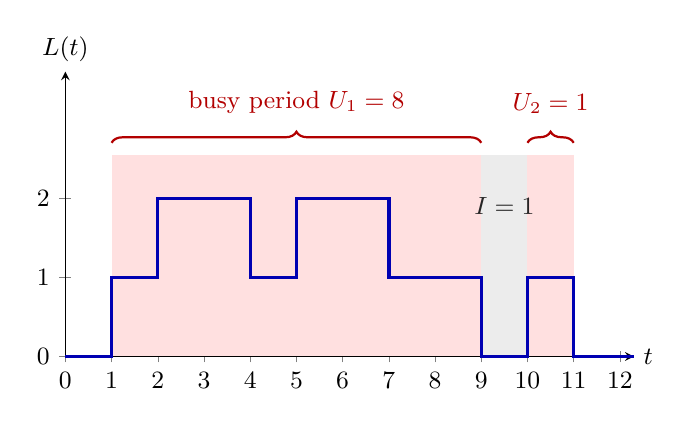
\begin{tikzpicture}[font=\small, >={Latex[length=2mm]}]
  \begin{axis}[
    axis lines=left, xmin=0, xmax=12.3, ymin=0, ymax=3.6,
    xtick={0,1,...,12}, ytick={0,1,2},
    xlabel={$t$}, ylabel={$L(t)$},
    xlabel style={at={(axis description cs:1,0)}, anchor=west},
    ylabel style={rotate=-90, at={(axis description cs:0,1)}, anchor=south},
    width=8.8cm, height=5.2cm, clip=false
    ]
    \fill[red!12] (axis cs:1,0) rectangle (axis cs:9,2.55);
    \fill[red!12] (axis cs:10,0) rectangle (axis cs:11,2.55);
    \fill[gray!15] (axis cs:9,0) rectangle (axis cs:10,2.55);
    \addplot[blue!70!black, very thick, const plot]
      coordinates {(0,0) (1,1) (2,2) (4,1) (5,2) (7,1) (9,0) (10,1) (11,0) (12.3,0)};
    \draw[red!70!black, thick, decorate, decoration={brace, amplitude=4pt}] (axis cs:1,2.7) -- (axis cs:9,2.7);
    \node[red!70!black, anchor=south] at (axis cs:5,2.95) {busy period $U_1=8$};
    \draw[red!70!black, thick, decorate, decoration={brace, amplitude=4pt}] (axis cs:10,2.7) -- (axis cs:11,2.7);
    \node[red!70!black, anchor=south] at (axis cs:10.5,2.95) {$U_2=1$};
    \node[gray!30!black] at (axis cs:9.5,1.9) {$I=1$};
  \end{axis}
\end{tikzpicture}
\end{document}
